\section{Het probleem:}
Onder de trappen is er onvoldoende verlichting, waardoor de treden niet goed zichtbaar zijn voor alle gasten. Dit gebrek aan zichtbaarheid kan leiden tot mogelijke ongelukken en letsel. Daarnaast heeft 1892 Eten \& Drinken aangegeven dat er behoefte is aan decoratie onder de bar om de sfeer te verbeteren en de ruimte aantrekkelijker te maken voor de gasten.

\subsection{De opdracht}
Traccy Solutions heeft de opdracht gekregen om de verlichting onder de trappen en bar aan te leggen bij 1892 Eten \& Drinken. Dit omvat het installeren van LED-strips met adresseerbare LED's om aantrekkelijke effecten te creëren die de ambiance van de zaal versterken en de kans op letsel te verkleinen. Deze verlichting zal worden aangestuurd via een speciale app voor een intuïtieve bediening.

\begin{figure}[!h]
\centering
\begin{subfigure}{.5\textwidth}
  \centering
  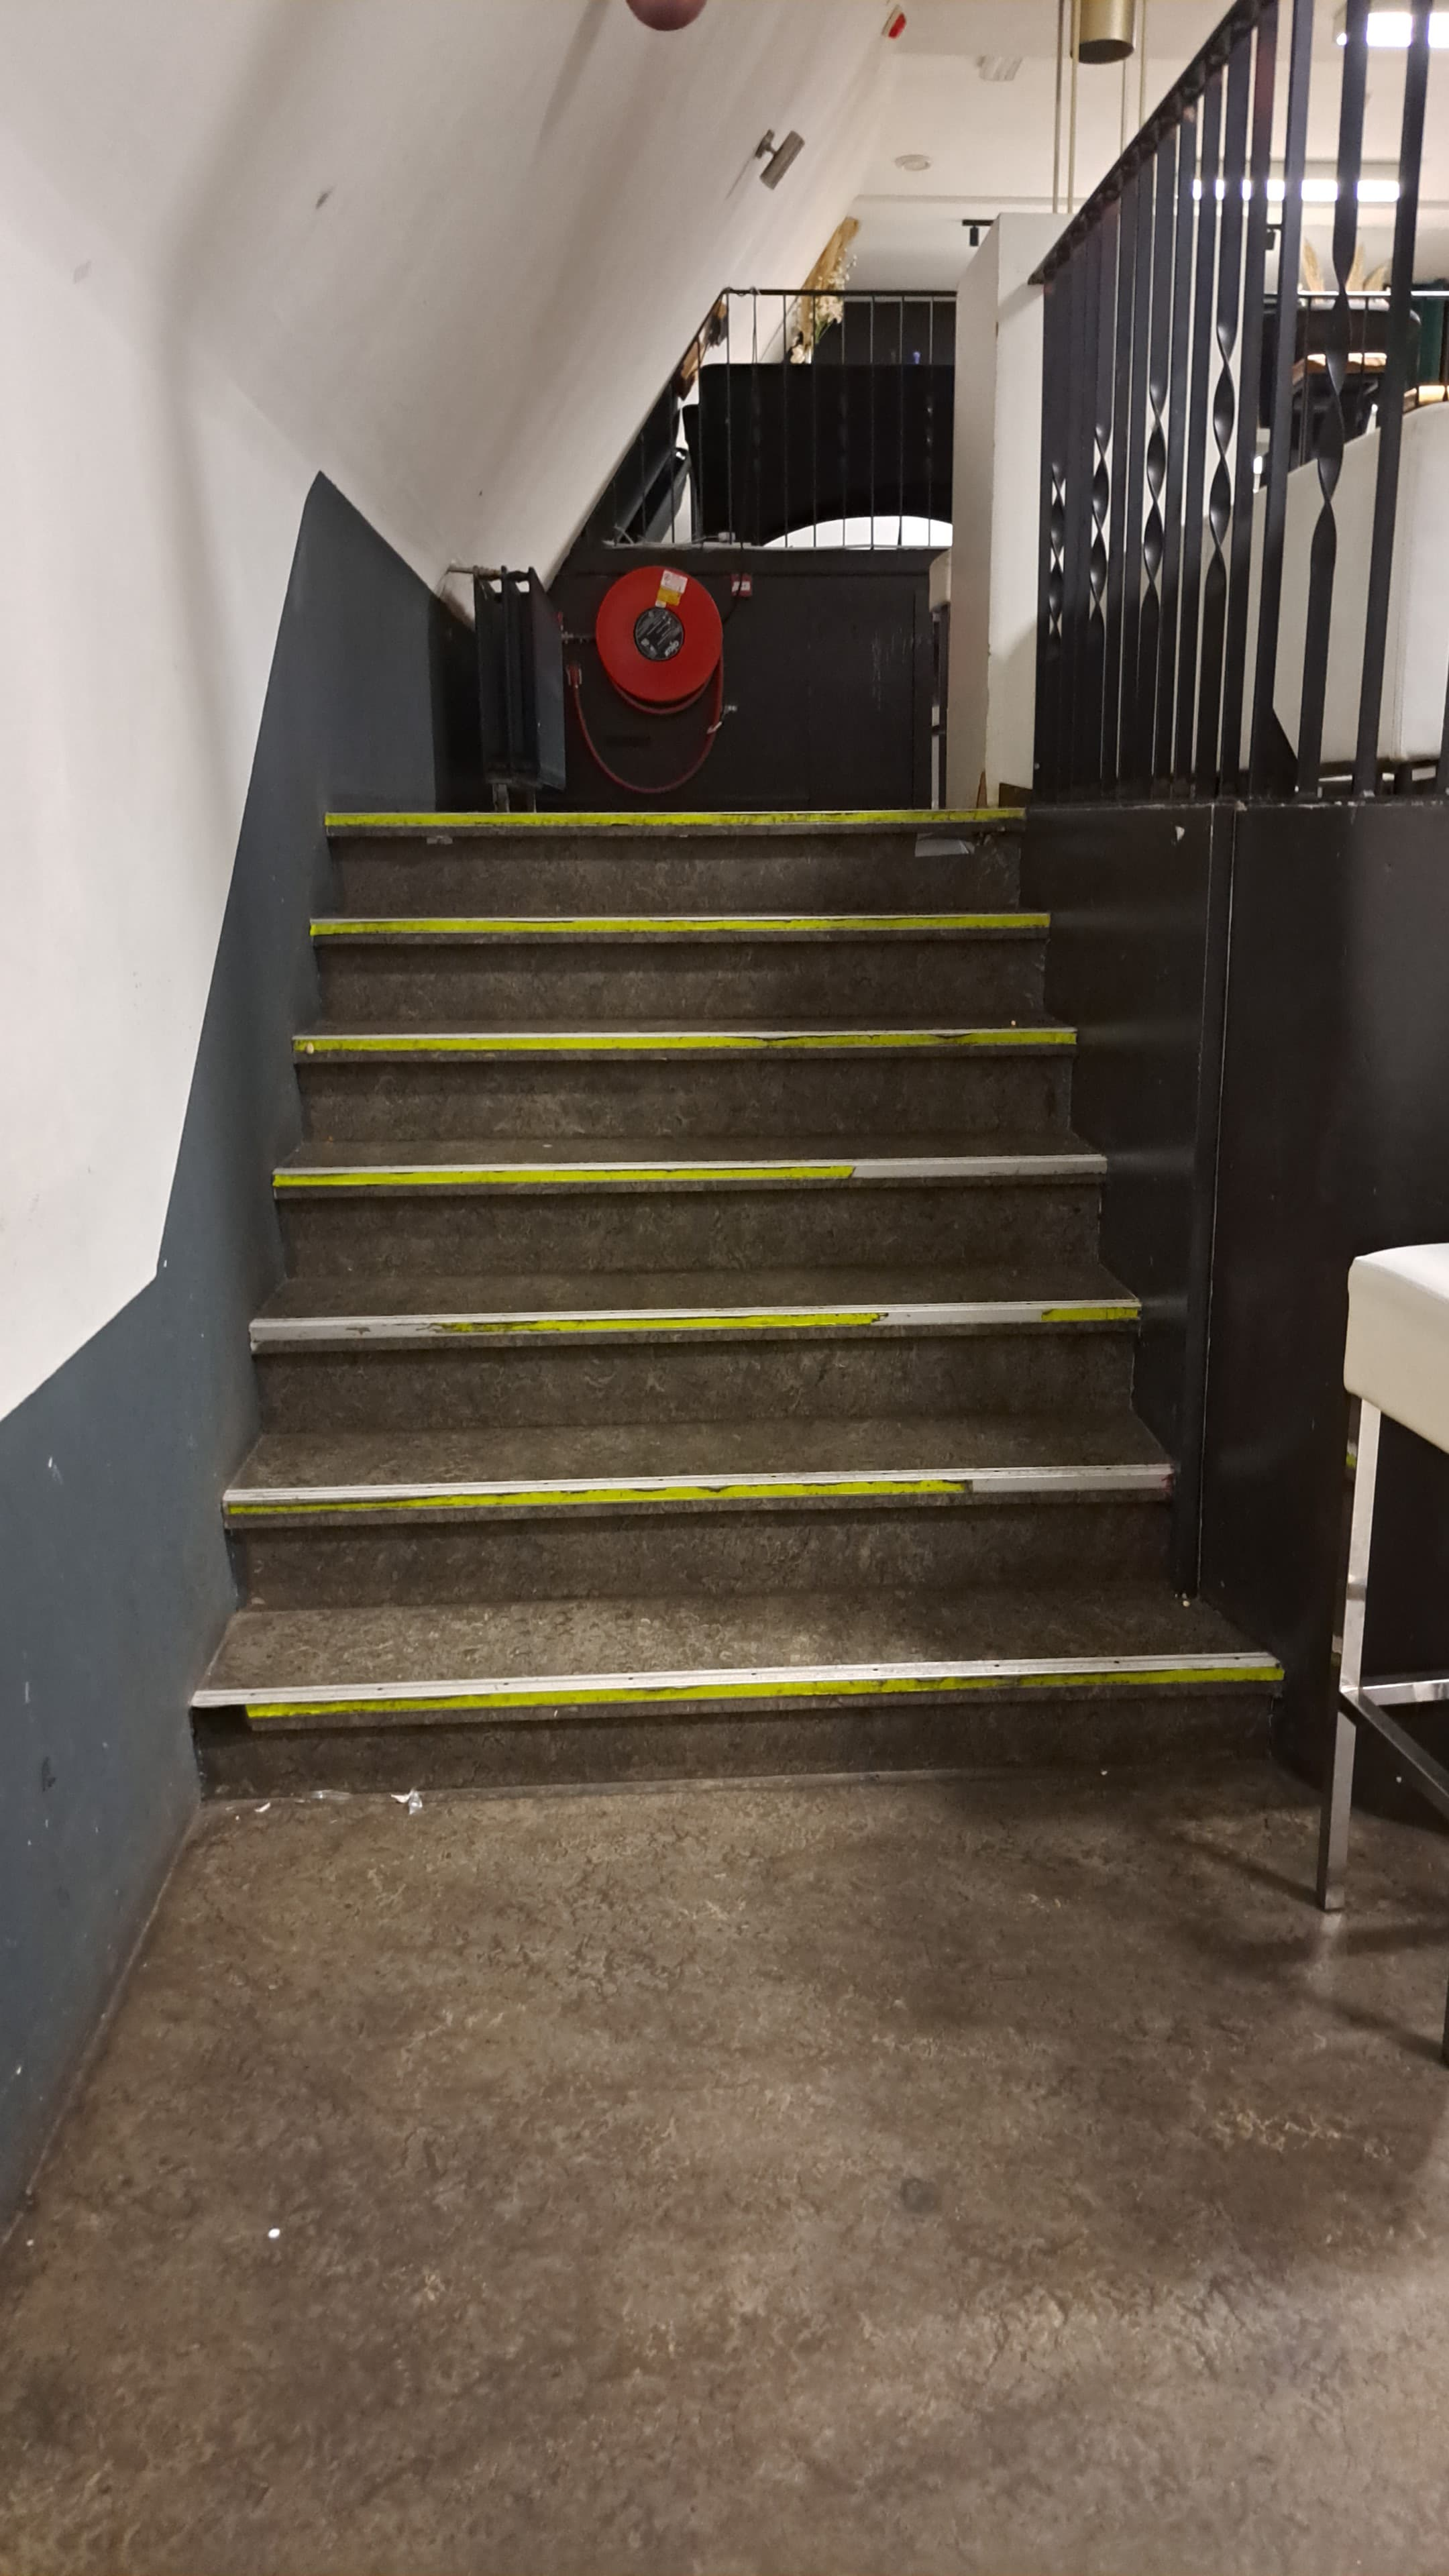
\includegraphics[width=.5\linewidth]{img/1892_trap.jpg}
  \caption{De trap in de huidige staat.}
  \label{fig:sub1}
\end{subfigure}%
\begin{subfigure}{.5\textwidth}
  \centering
  \includegraphics[width=.5\linewidth]{img/1892_trap_verlichting_render.png}
  \caption{Een schets van hoe de trap eruit komt te zien.}
  \label{fig:sub2}
\end{subfigure}
\caption{Een before and after tekening van de trap.}
\label{fig:test}
\end{figure}